\documentclass[a4paper,11pt]{article}
\usepackage[utf8]{inputenc}
\usepackage{minted}
\usepackage{amsmath}
\usepackage{float}
\usepackage[symbol]{footmisc}
\usepackage{graphicx}
\usepackage[toc,page]{appendix}

\graphicspath{{./figures/}}
\renewcommand{\thefootnote}{\fnsymbol{footnote}}

\title{\textbf{4. Linked List}}
\author{Kristiāns Vinters}
\date{Fall 2023}

\begin{document}
    \maketitle
    \section*{Introduction}

    I solved the assignment in Go. I used Go because I want to become more familiar with it. Source code and benchmark data is available on GitHub\footnote[1]{https://github.com/Phanty133/id1021/tree/master/4-linkedlist}.

    \section*{Implementation}

    There weren't any particular difficulties implementing linked lists in Go, as Go handles references with C-like pointers. I implemented the structure in a separate \texttt{llist} package.

    \begin{minted}{go}
type LinkedListItem[T comparable] struct {
    Head T
    next *LinkedListItem[T]
}

type LinkedList[T comparable] struct {
    first *LinkedListItem[T]
}
    \end{minted}

    I named the \texttt{next} and \texttt{first} members all-lowercase, as then they will be private to the package. I then added additional functions for reading just those fields from outside the package. It's the closest to a private setter, public getter you can have in Go. I did it like this to enforce that only internal functions can directly rearrange the list.

    \begin{minted}{go}
func (l *LinkedListItem[T]) Next() *LinkedListItem[T] {
    return l.next
}

func (l *LinkedList[T]) First() *LinkedListItem[T] {
    return l.first
}
    \end{minted}

    In addition to the required functions, I split off a \texttt{Last()} function from the \texttt{Append()} function, as that leads to a more readable implementation.

    \begin{minted}{go}
func (l *LinkedList[T]) Last() *LinkedListItem[T] {
    if l.first == nil {
        return nil
    }

    item := l.first

    for item.next != nil {
        item = item.next
    }

    return item
}

func (l *LinkedList[T]) Append(value T) *LinkedListItem[T] {
    item := &LinkedListItem[T]{Head: value}
    
    last := l.Last()
    last.next = item

    return item
}
    \end{minted}

    Implementing the linked list-based stack was also straightforward.

    \begin{minted}{go}
type LinkedListStack[T comparable] struct {
    list *LinkedList[T]
}

func (s *LinkedListStack[T]) Push(value T) {
    s.list.Add(value)
}

func (s *LinkedListStack[T]) Pop() (T, error) {
    item := s.list.First()

    if item == nil {
        var result T
        return result, errors.New("stack is empty")
    }

    s.list.first = item.next

    return item.Head, nil
}
    \end{minted}

    Both the array and linked list-based stacks have the same time complexities, however, the latter is not required to be contiguous in memory. As a result, there is no need to reallocate the entire stack when it grows.

    \section*{Benchmarking}

    I benchmarked the linked list and array by running them 250 times with a fixed size of 500 and changing sizes $\left\{10, 100, 1000, 5000, 10000, 15000\right\}$.

    \begin{figure}[H]
        \centering
        
        \begin{tabular}{c|c|c|c|c}
            Size & $t_\text{LL1}$, ms & $t_\text{Arr1}$, ms & $t_\text{LL2}$, ms & $t_\text{Arr2}$, ms \\
            \hline
            \hline
            10 & 0.006 & 0.001 & 0.142 & 0.001 \\
            \hline
            100 & 0.006 & 0.001 & 0.184 & 0.001 \\
            \hline
            1000 & 1.00 & 0.001 & 0.620 & 0.001 \\
            \hline
            5000 & 14.6 & 0.002 & 2.57 & 0.004 \\
            \hline
            10000 & 53.4 & 0.003 & 4.90 & 0.004 \\
            \hline
            15000 & 116 & 0.004 & 7.27 & 0.005 \\
        \end{tabular}

        \caption{Median times for (1) appending $n$ elements to a fixed number of elements, (2) appending a fixed number of elments to $n$ elements.}
    \end{figure}

    \begin{figure}[H]
        \centering
        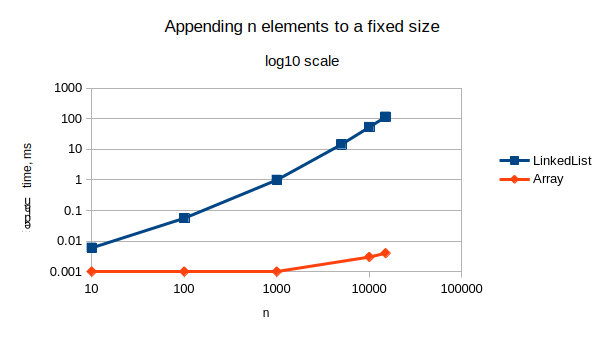
\includegraphics[width=\textwidth]{b1.png}
        \caption{Median time for benchmark 1}
        \label{fig:b1}
    \end{figure}

    \begin{figure}[H]
        \centering
        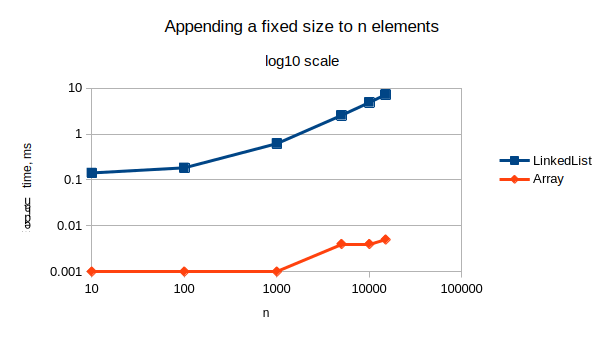
\includegraphics[width=\textwidth]{b2.png}
        \caption{Median time for benchmark 2}
        \label{fig:b2}
    \end{figure}

    From fig. \ref{fig:b1} and \ref{fig:b2} we can see that the linked list is slower than the array in both cases. This is because appending elements to the linked list is an operation with $O(n)$ time complexity, as the list has to be traversed to find the last element. The array, on the other hand, has $O(1)$ time complexity for appending elements, as it only has to increment the length counter and write the element to the next index.

    In fig. \ref{fig:b2}, a slight hump in the array execution time is visible around $n=5000$, as the number of appending elements exceeds the initial capacity of the array.

    There is also a significant difference in execution time between the first and second benchmark because when appending the fixed size, the entire linked list needs to be traversed less times.
\end{document}